% Setup - do not change
\documentclass[11pt]{article}

\usepackage[
    top=0.9in,
    left=0.9in,
    bottom=0.9in,
    right=0.9in
]{geometry}

\usepackage{parskip}

\usepackage[english]{babel}
\usepackage[utf8]{inputenc}
\usepackage{
    amsmath,
    amsthm,
    amssymb,
    graphicx,
    pdfpages,
    lipsum,
    hyperref
}

\usepackage[none]{hyphenat}
\usepackage{csquotes}
\usepackage{booktabs}
\usepackage{float}

\setlength\parindent{0pt}

% Bibliography
\usepackage[sorting=none]{biblatex}
\addbibresource{references_report.bib}


%%%%%%%%%%%%%%%%%%%%%%%%%%%%%%%%%%%%%%%%%%%%%%%%%%%%%%%%%%%%

\title{\textbf{Weather and Taxi Demand in New York City}}

\author{
Xinchen Zhou \\
Student ID: 1346673 \\
\href{https://github.com/bibobibobibobibo224/MAST30034-Project_1}{Github Repository}
}

\begin{document}

\maketitle


%%%%%%%%%%%%%%%%%%%%%%%%%%%%%%%%%%%%%%%%%%%%%%%%%%%%%%%%%%%%
% INTRODUCTION
%%%%%%%%%%%%%%%%%%%%%%%%%%%%%%%%%%%%%%%%%%%%%%%%%%%%%%%%%%%%

\section{Introduction}

Taxi demand varies across different areas of New York City and at different times of day. In addition, the weather also exerts a further influence on passengers’ decisions. In particular, when it rains, passengers are generally reluctant to walk or use public transport. Understanding how taxi demand changes under different weather conditions may therefore help taxi drivers better anticipate when and where passenger demand is likely to be higher.

This report investigates the relationship between the weather and taxi demand in NewYork city. The target audience are the yellow and green taxi drivers. By analyzing the temporal distribution of taxi demand under different weather conditions, the study aims to provide practical insights to help drivers reduce idle cruising and optimise vehicle positioning.

Taxi demand is measured as the number of valid passenger pickups recorded within each hour. The analysis first examines the spatial distribution of taxi pickups across New York City taxi zones under different weather conditions, than compared the hourly demand pattern between sunny and rainy weather. Finally, two statistical models, Linear Regression and XGBoost with a Poisson objective, are used to predict hourly taxi demand using weather condition, hour of day and day of week.

The analysis is observational and therefore focuses on associations rather than causal effects. 
Differences in taxi demand between Sunny and Rainy conditions may also get affected by other factors such as time of day, day of week and underlying travel patterns. These factors are therefore 
also included in the modelling stage.


\subsection{Data}

The primary dataset consists of Yellow and Green Taxi trip records published by the New York City 
Taxi and Limousine Commission (TLC) \cite{NYC TLC TripData}. The trip records contain information 
including pickup and drop-off timestamps, pickup and drop-off locations, trip distance and monetary 
values.

Both Yellow and Green Taxi records are included in the analysis to provide broader coverage of taxi 
activity across New York City. The two datasets contain comparable trip information and therefore can be combined after standardising their column names. Then study six consecutive months from 1st of December 2025 to 1st June 2026. This time range provides a sufficiently large dataset also covers both winter and spring for distributed processing with Pyspark. Also, during this time period, no significant events were observed that might lead to an inaccurate reflection of the general travel pattern.

Historical hourly weather observations for New York City were obtained from \cite{meteostat}. This data frame contained hourly weather data with parameters such as temperature, precipitation, weather as weather code (coco), and more. Each taxi trip is matched to the weather condition that corresponded to the recorded pickup time. 
In the main comparison, weather code 1 suggests \textit{Sunny} conditions, whereas many weather codes suggests \textit{Rainy} conditions, as shown in \textbf{Table-3}. This simplified comparison provides a clear distinction between dry and rainy conditions in the same timestamp. It avoids interpretation difficulties caused by combining several different forms of bad weather into one board category.

Hourly weather observations are assumed to be able to represent the weather condition experienced in NewYork during the corresponding hour. The counts for taxi pick ups implies taxi demand. The number of records for each dataset used in the study is summarized in Table-1.

\begin{table}[ht]
    \centering
    \caption{Datasets used in the study with record counts and feature dimensions.}
    \label{tab:datasets}

    \begin{tabular}{lrr}
        \toprule
        \textbf{Dataset} &
        \textbf{Number of Records} &
        \textbf{Number of Features} \\
        \midrule

        TLC Taxi Trip Records &
        23,563,503 &
        21 \\

        Historical Weather Data &
        4,366 &
        27 \\

        \bottomrule
    \end{tabular}
\end{table}


%%%%%%%%%%%%%%%%%%%%%%%%%%%%%%%%%%%%%%%%%%%%%%%%%%%%%%%%%%%%
% PREPROCESSING
%%%%%%%%%%%%%%%%%%%%%%%%%%%%%%%%%%%%%%%%%%%%%%%%%%%%%%%%%%%%

\section{Preprocessing}


\subsection{TLC Taxi Trip Records}

The TLC notes that trip records are supplied by authorised technology providers and are not guaranteed 
to be error-free \cite{nyctlc_tripdata}. Therefore preprocessing was performed to remove records that 
were incomplete, inconsistent or implausible before calculating taxi demand.

The following cleaning procedures were applied:

\begin{itemize}

    \item \textbf{Study period:}
    Yellow and Green Taxi records were combined and restricted to the period from 
    1 December 2025 to 31 May 2026. After this restriction, 23,563,503 trip records remained.

    \item \textbf{Missing and invalid trip records:}
    Records with missing pickup time, drop-off time, trip distance, fare amount, total amount 
    or tip amount were removed. And for the 3 monetary element only positive records were decided to kept since negative values likely result from sensor or database errors. Trips were also required to have a drop-off time later than the pickup time, positive trip distance, and trip duration between 2 minutes and 8 hours with the same reason like the monetary elements. After these validity checks, 22,326,870 trips remained.

    \item \textbf{Implausible average speed:}
    Average trip speed was calculated from trip distance and trip duration. Trips with non-positive average speed or speed above 75 miles per hour were removed since in New york the maximum speed limit is 65 mp/h \cite{nyc311_speedlimits} on highway so a conservative range is applied. This reduced the dataset to 22,322,930 trips.

    \item \textbf{Extreme trip duration:}
    Since reasonable trip duration depends strongly on trip distance, trips were divided into 
    distance groups. Within each group, an upper outlier threshold of
    
    \[
    Q_3 + 3IQR
    \]
    
    was applied to remove extreme duration outliers while retaining legitimate long-duration trips. 22,121,294 data entries remain after this filtering step.
    
    \item \textbf{Extreme low-speed observations:}
    A log transformation is applied on average speed to identify extremely low speed observations using a $3IQR$ lower bound. 21,995,162 trips remain after removing these observations.

    \item \textbf{Pickup location validation:}
    Pickup-zone identifiers were matched with the NYC TLC taxi-zone lookup table and only zones which belong to the 5 New York city boroughs were retained. 21,966,943 valid taxi trips were left after 28,219 records was removed due to invalid pickup-zone identifiers.

\end{itemize}

Overall, 1,596,560 records were removed from the original dataset, representing approximately 6.78\% of the 23.56 million initial trip records. This cleaning process aims to have removed records which might affect hourly demand estimates or spatial comparisons.


\begin{table}[ht]
    \centering
    \caption{Taxi preprocessing record counts.}
    \label{tab:taxi_preprocessing}

    \begin{tabular}{lrr}
        \toprule

        \textbf{Preprocessing Stage}
        & \textbf{Rows Remaining}
        & \textbf{Rows Removed} \\

        \midrule

        Study-period filter
        & 23,563,503
        & -- \\

        Missing and invalid trip filter
        & 22,326,870
        & 1,236,633 \\

        Speed filter
        & 22,322,930
        & 3,940 \\

        Distance-group duration IQR filter
        & 22,121,294
        & 201,636 \\

        Log-speed IQR filter
        & 21,995,162
        & 126,132 \\

        Valid NYC pickup-zone join
        & 21,966,943
        & 28,219 \\

        \bottomrule
    \end{tabular}
\end{table}


After preprocessing and location validation, variables used only for data-quality checks, such as 
trip duration, trip distance and average speed, were removed. The remaining taxi variables used 
for demand analysis were pickup timestamp, hourly pickup timestamp and pickup taxi zone.


\subsection{Historical Weather Data}

Hourly historical weather data for 2025 and 2026 were combined and restricted to the same period 
as the taxi dataset. Since my topic is to assess the condition of weather so only weather hour and the weather code 'coco' which  indicates the specific weather condition recorded by the meteorological station was retained.

A corresponding hourly timestamp was than created for the weather records and converted to New York 
local time so that the weather observations could be matched correctly with taxi pickup times. 
Only the variables required for the analysis were retained.

For the primary weather comparison, Meteostat weather code 1 was classified as \textit{Sunny}. 
Rain-related weather codes were classified as \textit{Rainy}. The resulting classification was used 
for the geospatial comparison, hourly demand analysis and statistical modelling. The 8 distinct weather type contained in the weather csv with its corresponding weather code is showed below.

\begin{table}[ht]
    \centering
    \caption{Weather condition categories and corresponding weather codes.}
    \label{tab:weather_categories}

    \begin{tabular}{p{0.18\textwidth} p{0.72\textwidth}}
        \toprule
        \textbf{Category} & \textbf{Conditions (with codes)} \\
        \midrule

        Sunny &
        Clear (1) \\

        Rainy &
        Light Rain (7), Rain (8), Heavy Rain (9), Freezing Rain (10),
        Heavy Freezing Rain (11), Sleet (12), Heavy Sleet (13),
        Light Snowfall (14), Rain Shower (17), Heavy Rain Shower (18) \\

        \bottomrule
    \end{tabular}
\end{table}


%%%%%%%%%%%%%%%%%%%%%%%%%%%%%%%%%%%%%%%%%%%%%%%%%%%%%%%%%%%%
% ANALYSIS AND GEOSPATIAL VISUALISATION
%%%%%%%%%%%%%%%%%%%%%%%%%%%%%%%%%%%%%%%%%%%%%%%%%%%%%%%%%%%%

\section{Analysis and Geospatial Visualisation}

\subsection{Spatial Taxi Demand under Different Weather Conditions}

\begin{figure}[H]
    \centering

    \begin{minipage}{0.48\textwidth}
        \centering

        \textbf{Spatial Distribution of NYC Taxi Demand}\\
        \textbf{under Sunny Weather}

        \vspace{0.1cm}

        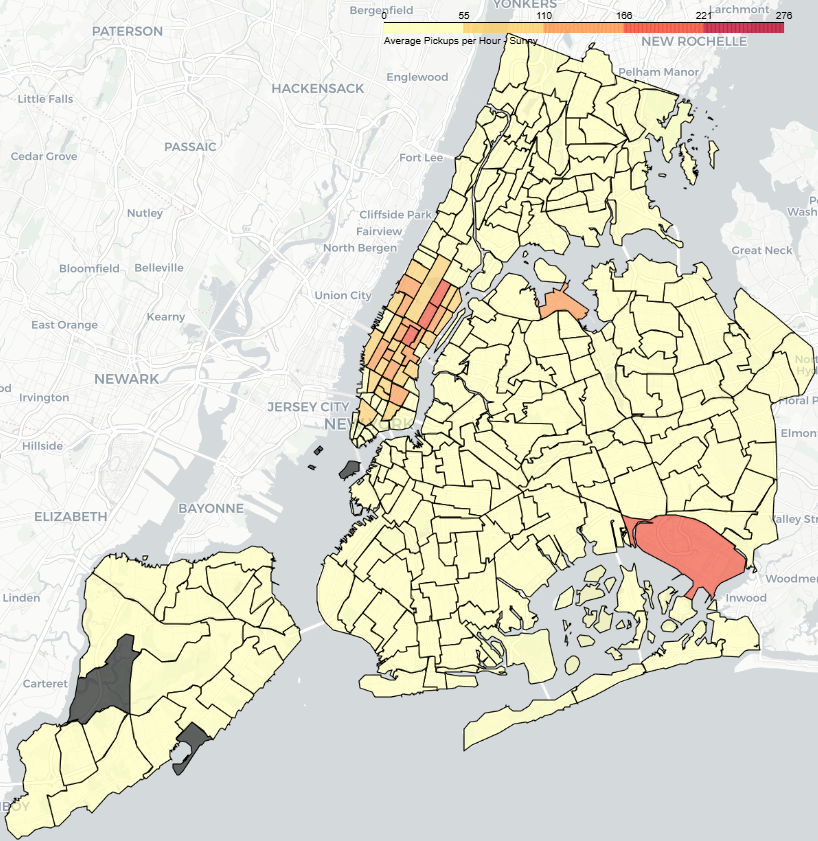
\includegraphics[width=\linewidth]{Sunny.png}

        \vspace{0.1cm}

        \small
        \textbf{(a)} Average taxi pickups per hour by TLC Taxi Zone
        under Sunny weather.
    \end{minipage}
    \hfill
    \begin{minipage}{0.48\textwidth}
        \centering

        \textbf{Spatial Distribution of NYC Taxi Demand}\\
        \textbf{under Rainy Weather}

        \vspace{0.1cm}

        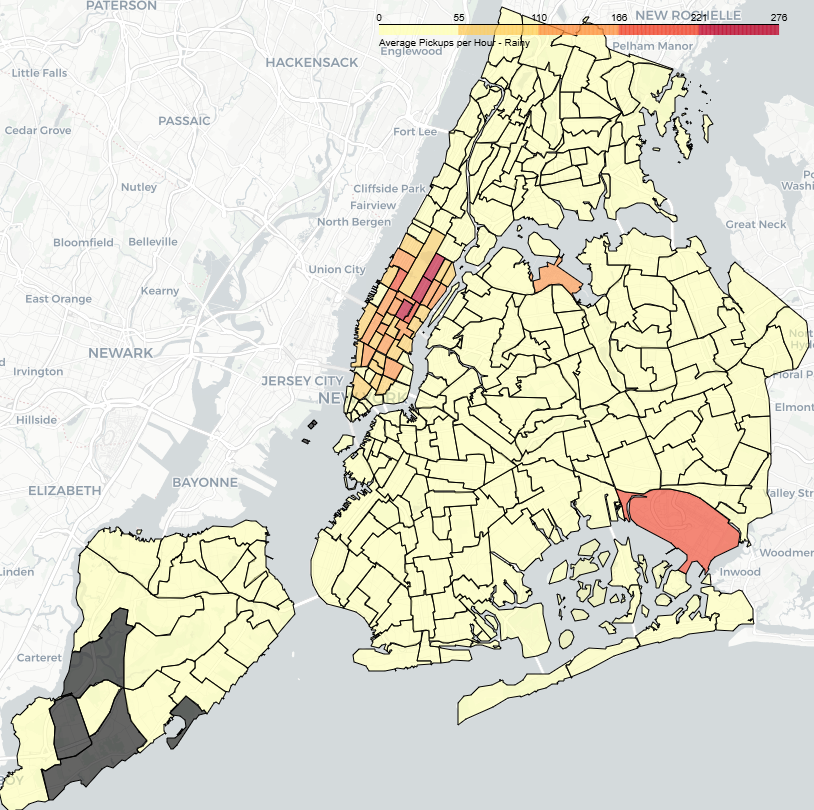
\includegraphics[width=\linewidth]{Rainy.png}

        \vspace{0.1cm}

        \small
        \textbf{(b)} Average taxi pickups per hour by TLC Taxi Zone
        under Rainy weather.
    \end{minipage}

    \caption{Comparison of average hourly taxi demand under
    (a) Sunny and (b) Rainy weather conditions in New York City.
    Both maps use the same colour scale.}
    \label{fig:weather_maps}
\end{figure}

From Figure~\ref{fig:weather_maps}, taxi demand is spatially concentrated under both weather conditions, particularly in Manhattan and the airport area in Queens,while
many outer-borough zones show relatively low demand.The overall spatial pattern is
similar between Sunny and Rainy weather, although almost half high-demand taxi zones showed a increased pick up intensity during rainy weather compare to when it is sunny. This suggests that rainy conditions are associated with higher demand within the existing high-demand areas rather than a change in where taxi demand occurs.

%%%%%%%%%%%%%%%%%%%%%%%%%%%%%%%%%%%%%%%%%%%%%%%%%%%%%%%%%%%%
% HOURLY DEMAND ANALYSIS
%%%%%%%%%%%%%%%%%%%%%%%%%%%%%%%%%%%%%%%%%%%%%%%%%%%%%%%%%%%%

\subsection{Hourly Taxi Demand under Different Weather Conditions}

\begin{figure}[H]
    \centering
    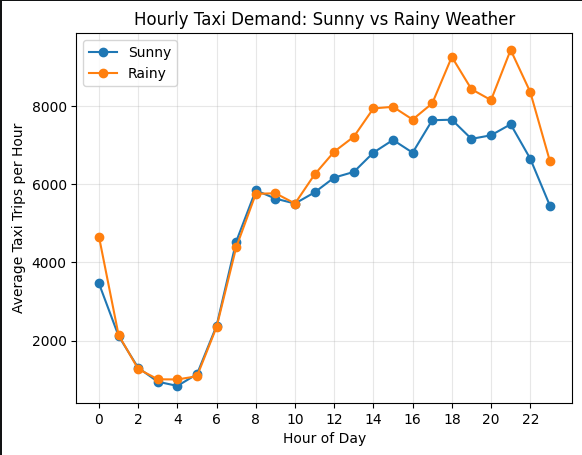
\includegraphics[width=0.78\textwidth]{hourly_demand.png}
    \caption{Average hourly taxi demand under Sunny and Rainy weather conditions.}
    \label{fig:hourly_demand}
\end{figure}

From Figure~\ref{fig:hourly_demand}, a similar daily demand pattern is showed for both sunny and rainy days. Taxi demand reaches its lowest level at approximately 3-5 AM
before increasing throughout the morning. Rainy conditions generally show higher
average taxi demand during several daytime and evening hours, although the overall
shape of the two curves remains similar.

Compare to the variation of taxi demands between sunny and rainy days, the substantial variation in demand across hours of the day suggests that time of day
may be more strongly associated with taxi demand than weather condition. Since in the very early morning due to not many people is getting taxi trips the demand can hardly be very different. But weather still appears to contribute additional variation, particularly during some daytime and evening periods.

%%%%%%%%%%%%%%%%%%%%%%%%%%%%%%%%%%%%%%%%%%%%%%%%%%%%%%%%%%%%
% MODELLING
%%%%%%%%%%%%%%%%%%%%%%%%%%%%%%%%%%%%%%%%%%%%%%%%%%%%%%%%%%%%

\section{Modelling}

Two contrasting models were used to predict hourly taxi demand: Linear Regression
and XGBoost with a Poisson objective. The response variable was the hourly number
of taxi trips, \texttt{trip\_count}. The predictors were weather condition, hour of
day and day of week. Weather was represented by a binary variable where Rainy was
coded as 1 and Sunny as 0. Hour of day and day of week were treated as categorical
variables and one-hot encoded before modelling.

The data was split chronologically rather than randomly to evaluate the ability od the models to predict future demand. Approximately 83.3\% of the six-month study
period which is from December 2025 to April 2026 was used for training. While the remaining
16.7\%, corresponding to May 2026, was held out for testing. Model performance was evaluated using three standard regression metrics: Mean
Absolute Error (MAE), Root Mean Squared Error (RMSE), and $R^2$. Together, these
metrics assess the magnitude of prediction errors and the proportion of variation
in hourly taxi demand explained by the models.

\subsection{Linear Regression}

Linear Regression was used as an interpretable baseline model. The model can be
represented as

\[
\widehat{\text{Demand}}_t =
\beta_0 +
\beta_1 \text{Rain}_t +
\sum_h \gamma_h \text{Hour}_{h,t} +
\sum_d \delta_d \text{Day}_{d,t}.
\]

This model assumes that the effects of weather, hour of day and day of week are
additive. One category from hour of day and day of week is omitted during one-hot
encoding and therefore acts as the reference category.

The estimated coefficient for the Rainy indicator was 643.76. Under the condition of keeping daily hours and weekly days constant, this model associates approximately 644 additional taxi trips per hour under rainy conditions compared to sunny conditions. This coefficient describes the correlation observed in the data and should not be interpreted as a causal effect of rainfall.


\subsection{XGBoost with Poisson Objective}

Since hourly taxi demand is a non-negative count, XGBoost was fitted
using a Poisson objective. Let $Y_i$ denote the number of taxi trips during hour
$i$. The expected hourly demand is represented as

\[
\mathbb{E}[Y_i \mid X_i] = \lambda_i,
\]

where $X_i$ contains the weather condition, hour of day and day of week.
Under the Poisson objective, the expected count can be expressed through a log link as

\[
\log(\lambda_i) = F(X_i),
\]

where $F(X_i)$ is the prediction obtained from a group of decision trees.
XGBoost builds these trees sequentially, and each new tree will improve the prediction
based on the errors of the previous trees made. This allows the model to capture nonlinear
relationships and interactions between the predictors which may not be represented
by the Linear Regression model.

The model used 200 trees with a maximum tree depth of 5 and a learning rate of 0.05, aimed to control the complexity of the model.

%%%%%%%%%%%%%%%%%%%%%%%%%%%%%%%%%%%%%%%%%%%%%%%%%%%%%%%%%%%%
% RESULTS
%%%%%%%%%%%%%%%%%%%%%%%%%%%%%%%%%%%%%%%%%%%%%%%%%%%%%%%%%%%%

\section{Results and Discussion}

\subsection{Model Performance}

Model performance on the May 2026 test period was assessed using Mean Absolute Error
(MAE), Root Mean Squared Error (RMSE) and $R^2$. The results are shown in
Table~\ref{tab:model_results}.

\begin{table}[H]
    \centering
    \caption{Model performance on the May 2026 test data.}
    \label{tab:model_results}
    \begin{tabular}{lccc}
        \toprule
        Model & MAE & RMSE & $R^2$ \\
        \midrule
        Linear Regression & 1024.15 & 1375.02 & 0.7500 \\
        XGBoost Poisson & 1014.83 & 1399.17 & 0.7412 \\
        \bottomrule
    \end{tabular}
\end{table}

The two models produced similar predictive performance. XGBoost achieved a slightly
lower MAE, with an average absolute prediction error of approximately 1,015 trips
per hour compared with 1,024 for Linear Regression. However, Linear Regression
achieved a lower RMSE and a slightly higher $R^2$. Its $R^2$ of 0.750 indicates
that approximately 75\% of the variation in hourly taxi demand in the test period
was accounted for by the included predictors.

The small difference between the two models suggests that introducing a more
flexible tree-based model did not substantially improve prediction for the variables
used in this study. The strong performance of the simpler Linear Regression model
also suggests that hour of day, day of week and weather condition already capture
a substantial proportion of the variation in hourly taxi demand.


\subsection{Weather and Taxi Demand}

In May 2026, the average demand observed during Sunny conditions
was 4,830 taxi trips per hour, and 5,427 under Rainy conditions - approximately 12.37\% increase when it rains.

This result is consistent with the positive Rainy coefficient from the
Linear Regression model. It implies that at certain times of day, predicted taxi demand can be higher due to the rainy condition. And this difference is considered as an association, which is different to other unobserved factors that may vary between Sunny and Rainy periods.


\subsection{Feature Importance}

Figure~\ref{fig:feature_importance} shows the 10 most important features identified
by the XGBoost model using gain-based feature importance.

\begin{figure}[H]
    \centering
    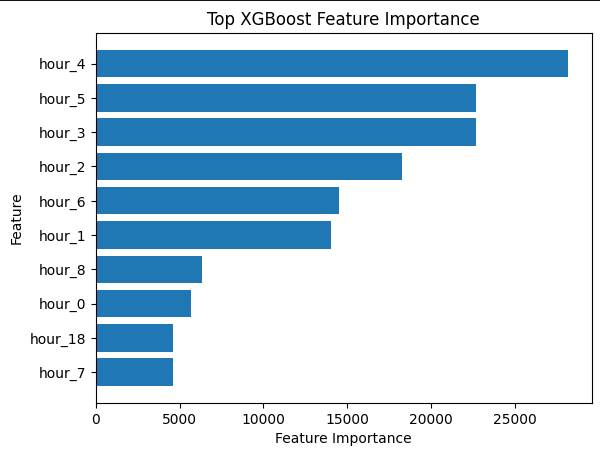
\includegraphics[width=0.75\textwidth]{feature_importance.png}
    \caption{Top ten XGBoost features ranked by gain-based feature importance.}
    \label{fig:feature_importance}
\end{figure}

The most important predictor is the hour of day. Hours 2-6 AM corresponds to the strong overnight decline in taxi demand observed previously in Figure~\ref{fig:hourly_demand}. This predictor is useful in distinguishing low-demand periods.

The Rainy indicator had a feature-importance value of 295.53 and was ranked 26th in the most important predictor plot shown in code. This suggests that although Rainy conditions are associated with higher taxi demand, time of day provides substantially more information for predicting the overall level of hourly demand. This is consistent
with the hourly analysis before, where variation across the different hour in a day was considerably larger than the difference between Sunny and Rainy conditions.


%%%%%%%%%%%%%%%%%%%%%%%%%%%%%%%%%%%%%%%%%%%%%%%%%%%%%%%%%%%%
% RECOMMENDATIONS
%%%%%%%%%%%%%%%%%%%%%%%%%%%%%%%%%%%%%%%%%%%%%%%%%%%%%%%%%%%%

\section{Recommendations}

The results provide two practical recommendations for NYC drivers.

One, drivers should pay more attention to \textbf{the specific time periods of the day} relative to the rain conditions, as displayed by the importance of XGBoost features. There are significant differences in the demand throughout the day especially when in the morning.

Two, \textbf{rainy days can be regarded as additional demand signals, rather than the main positioning strategy}. During the May test period, the average demand on rainy days was approximately 12.37\% higher than that on sunny days. On the other hand, spatial analysis showed that the main high-demand areas remained similar between sunny and rainy days. Therefore, when it rains, drivers do not need to completely shift to other areas. Instead, when the rainy days coincide with the usually busy periods, they can prioritize the existing high-demand areas, especially the areas around airports in Manhattan and Queens.

These recommendations relate to the order-taking demands and potential order-taking opportunities, but they do not directly imply that drivers will earn more, as income also depends on factors such as the distance of the trip, the fare structure, traffic conditions, and operating costs.


%%%%%%%%%%%%%%%%%%%%%%%%%%%%%%%%%%%%%%%%%%%%%%%%%%%%%%%%%%%%
% CONCLUSION
%%%%%%%%%%%%%%%%%%%%%%%%%%%%%%%%%%%%%%%%%%%%%%%%%%%%%%%%%%%%

\section{Conclusion}

In this report, we investigated the relationship between weather conditions and Yellow and Green taxi demand in New York City from December 2025 to May 2026. The analysis combined NYC TLC taxi trip records with hourly weather data and examined spatial and hourly demand patterns. It showed that taxi demand remained concentrated in Manhattan and airport-related areas in Queens independent of rain. However, several high-demand areas showed higher pickup intensity during Rainy periods. The hourly analysis reviewed that demand drastically changed during the day, with particularly low demand in the morning. Furthermore, Linear Regression and XGBoost were used to predict hourly taxi demand. The Linear Regression model achieved an $R^2$ of 0.750, while the XGBoost model achieved an $R^2$ of 0.741, indicating similar predictive performance. Rainy periods were associated with higher average hourly demand; whereas, the XGBoost feature importance showed that the hour of day substantially help with making predictions relative to the Rain indicator. Overall, the results suggest that drivers should consider time over the rain condition. They should also favour certain locations as their main base of operations. Then, they can take in the rain condition, since areas originally with high demand will result in a even higher demand when its raining, especially during the day.  Future research could incorporate additional factors such as public holidays, major events and traffic conditions to further explain variations in taxi demand.



%%%%%%%%%%%%%%%%%%%%%%%%%%%%%%%%%%%%%%%%%%%%%%%%%%%%%%%%%%%%
% REFERENCES
%%%%%%%%%%%%%%%%%%%%%%%%%%%%%%%%%%%%%%%%%%%%%%%%%%%%%%%%%%%%


\printbibliography

\end{document}

